%----------------------------------------------------------------------------
%----------------------------------------------------------------------------
%				    	SETUP
%----------------------------------------------------------------------------
%----------------------------------------------------------------------------

\documentclass[11pt]{article}

%----------------------------------------------------------------------------
%			  	   PACKAGES
%----------------------------------------------------------------------------

%%%%%%%%%%%%%%%%%%%%%%%
% 	  Packages
%%%%%%%%%%%%%%%%%%%%%%%

%% Fonts and Symbols
%% --------------------------
\usepackage{
			amsmath,			% math operators
			amssymb,			% math symbols
%			amsthm,				% theorem environment
			soul,				% strike through with \st{}
			xcolor,				% color!
%			xfrac,				% fancy fractions
}		

%% Graphics
%% --------------------
\usepackage{
			graphicx,			% allows insertion of images
			subfigure,			% allows subfigures (a), (b), etc.
}				
\graphicspath{ {graphics/} }	% (graphicx) relative path to graphics folder				

%% Tables
%% --------------------------
\usepackage{
			booktabs,			% better tables, discourages vertical rulings
			multicol,			% allow multi columns
%			tocloft,			% finer control over TOC; enabled below due to subfigure conflict
}
%\usepackage[subfigure]{tocloft}
%\addtocontents{toc}{\cftpagenumbersoff{subsubsection}} % turn off subsubsection page numbers in ToC

%% Layout Alteration
%% --------------------------
\usepackage{			
%			caption,			% line breaks in captions with \\
%			changepage,			% change margins for PARTS of pages with (adjustwidth)
			fancyhdr,			% see config in LAYOUT AND STYLING
			framed,				% nice boxes; used in Supervisor's Approval
%			fullpage,			% set full page margins
			geometry,			% change the margins for specific PAGES
%			lastpage,			% used with (fancyhdr)
			parskip,			% disable indents
%			pdflscape,			% ???
			rotating,			% sideways figures
}
\geometry{						% specify page size options for (geometry)
			a4paper, 			% paper size
			hmargin=1in,		% horizontal margins
			vmargin=1in,		% vertical margins
}	


%% Units
%% --------------------------
\usepackage{
			siunitx,			% has S (decimal align) column type
}
\sisetup{input-symbols = {()},  % do not treat "(" and ")" in any special way
		group-digits  = false, 	% no grouping of digits
%		 load-configurations = abbreviations,
%		 per-mode = symbol,
}

%% Misc
%% --------------------------
\usepackage{
			enumitem,			% better control of enumerations, descriptions, etc
}



%----------------------------------------------------------------------------
%		     MACROS AND COMMANDS
%----------------------------------------------------------------------------

% Defines a new command for the horizontal lines, change thickness here
\newcommand{\HRule}{\rule{\linewidth}{0.5mm}} 

% scientific notation  use \e
\providecommand{\e}[1]{\ensuremath{\times 10^{#1}}}

% override S column type with centered text column
\newcommand{\textcol}[1]{\multicolumn{1}{c}{#1}}

% easy unit spacing in math mode
\providecommand{\units}[1]{\;\text{#1}}

%----------------------------------------------------------------------------
%----------------------------------------------------------------------------
%				   DOCUMENT
%----------------------------------------------------------------------------
%----------------------------------------------------------------------------

\begin{document}

%----------------------------------------------------------------------------
%				    TITLE PAGE
%----------------------------------------------------------------------------

\begin{titlepage}

\center
 
% Header
\textsc{\LARGE University of Victoria}\\[1cm] 	% Name of your university/college
\textsc{\Large CENG 241}\\[0.5cm] 			% Major heading such as course name
\textsc{\large Digital Design I}\\[0.5cm] 		% Minor heading such as course title


% Lab Title
\HRule \\[0.4cm]
{ \huge \bfseries Lab 1 - Digital Instrumentation, Basic Digital Components and Circuits}\\[0.2cm] % Title of your document
\HRule \\[1.5cm]
 
 
%Lab Instructor Details
\begin{minipage}{0.7\textwidth}
\begin{flushleft} 

\large\emph{Instructor:} \\
Dr. Amirali \textsc{Baniasadi} \\
\vspace{12 pt}
\emph{Teaching Assistant:} \\
Grace \textsc{Hui}

\end{flushleft}
\end{minipage}
~
%% No content here, but it keeps the alignment of the instructor/TA
%% box correct.
%% Consider revising.
\begin{minipage}{0.1\textwidth}
\begin{flushright} \large
%Dr. Barbara \textsc{Sawicka} \\
\vspace{12 pt}
%\emph{Teaching Assistant:} \\
%Vahid \textsc{Moradi}
\end{flushright}
\end{minipage}\\[2cm]


% Lab members
\Large Yves \textsc{Senechal}
\large V00213837	\\
\Large Tyler \textsc{Stephen}
\large V00812021	\\
A01 - B03\\[1.5cm] 


% Date
{\large June 1, 2015}\\ % Date, change the \today to a set date if you want to be precise

% Logo
\begin{figure}[b]	 % put logo at bottom of the page
	\centering
	\includegraphics[scale=0.3]{UVic_logo}
\end{figure}

\end{titlepage}

%----------------------------------------------------------------------------
%				    BODY
%----------------------------------------------------------------------------

\section{Introduction}

\section{Voltage Regulators}
\begin{table}[h]
	\centering
	\begin{tabular}{ @{} S S S S S S @{} }
		\toprule
		\textcol{$V_{in}$ (V)} &
			\textcol{$V_{out}$ (V)} &
			\textcol{$I_{in}$ (mA)} &
			\textcol{$I_{out}$ (mA)} &
			\textcol{$P$ (mW)} &
			\textcol{$T$ ($^{\circ}$C)} \\
		\midrule
		0.0	& 2\e{-5}	& 2\e{-4}	& 2\e{-4}	& & 22.9 \\
		1.0	& 1.5\e{-5}	& 2\e{-4}	& 2\e{-4}	& & 22.9 \\
		2.0	& 4.3\e{-4}	& 6\e{-4}	& 6\e{-4}	& & 23.3 \\
		3.0	& 1.5913	& 1.599		& 1.599		& & 23.0 \\
		4.0	& 2.5057	& 2.5143	& 2.5143	& & 23.2 \\
		5.0	& 3.662		& 3.6758	& 3.6758	& & 23.4 \\
		6.0	& 4.689		& 4.7083	& 4.7083	& & 23.8 \\
		7.0	& 4.992		& 5.0129	& 5.0129	& & 24.1 \\
		8.0	& 4.904		& 4.9252	& 4.9252	& & 24.8 \\
		9.0	& 4.845		& 4.8655	& 4.8655	& & 25.7 \\
		10.0& 4.815		& 5.053		& 5.053		& & 25.8 \\
		11.0& 4.777		& 5.050		& 5.050		& & 26.3 \\
		12.0& 4.759		& 5.0217	& 5.0127	& & 27.2 \\
		\bottomrule
	\end{tabular}
	\caption{Voltage, current and temperature response of LM7805 5V regulator}
	\label{table:regulator}
\end{table}

{\em The range of voltages where the regulator voltage output is constant}

{\em What happens when the regulator is short circuited?}

\section{Signal damping}
{\em waveforms of under, over, critically damped waves}

\begin{sidewaysfigure}[h]
	\centering
	\subfigure[Over damping]
	{
		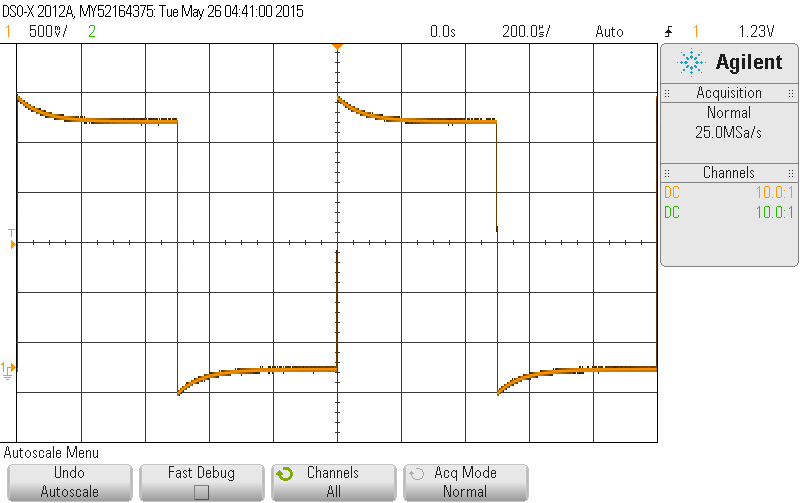
\includegraphics[width=0.475\textwidth, draft=false]{overdamped}
	}
	\subfigure[Under damping]
	{
		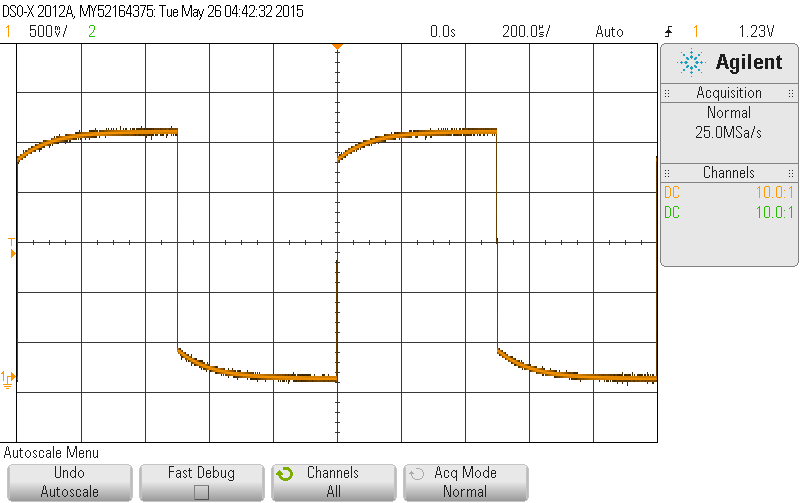
\includegraphics[width=0.475\textwidth, draft=false]{underdamped}
	}
	\subfigure[Critical damping]
	{
		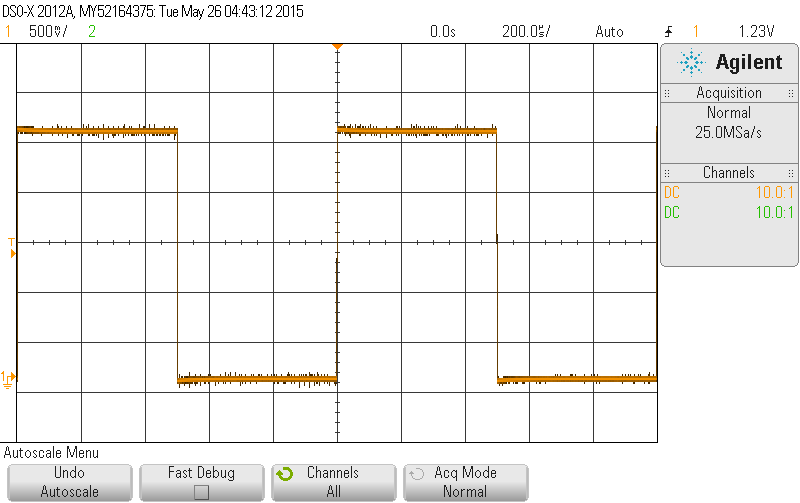
\includegraphics[width=0.475\textwidth, draft=false]{critdamped}
	}
	\caption{Waveforms representative of different levels of damping for a square wave}
	\label{fig:damping}
\end{sidewaysfigure}

{\em rise and fall time of critically damped wave}
\begin{figure}[h]
	\centering
	\subfigure[Rise time]
	{
		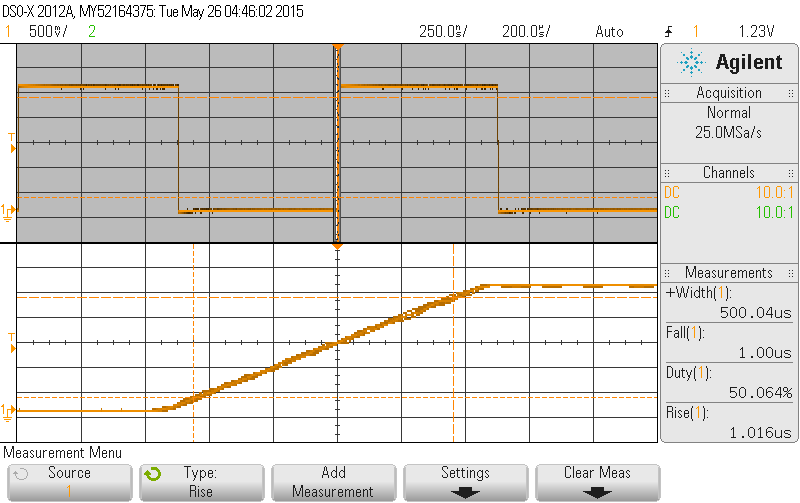
\includegraphics[width=0.95\textwidth, draft=false]{risetime}
	}
	\subfigure[Fall time]
	{
		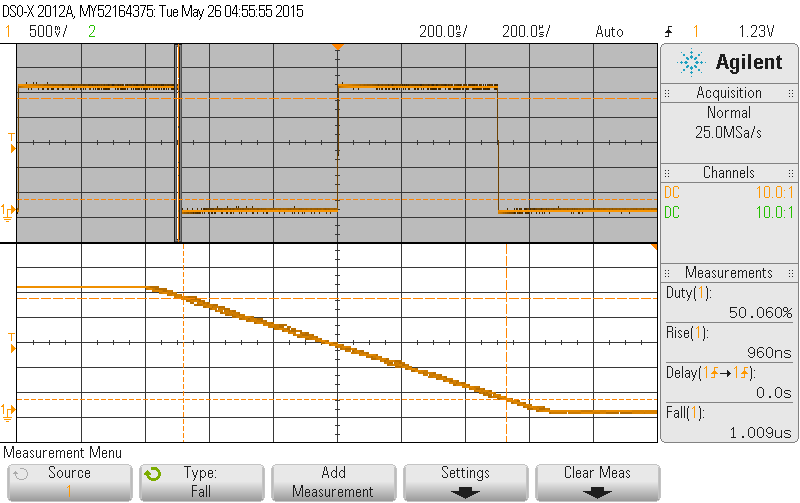
\includegraphics[width=0.95\textwidth, draft=false]{falltime}
	}
	\caption{Opposite edges of a critically damped square wave}
	\label{fig:rise_fall}
\end{figure}

\section{LEDs and Inverters}
{\em When is the LED lit?}
\begin{figure}[h]
	\centering
	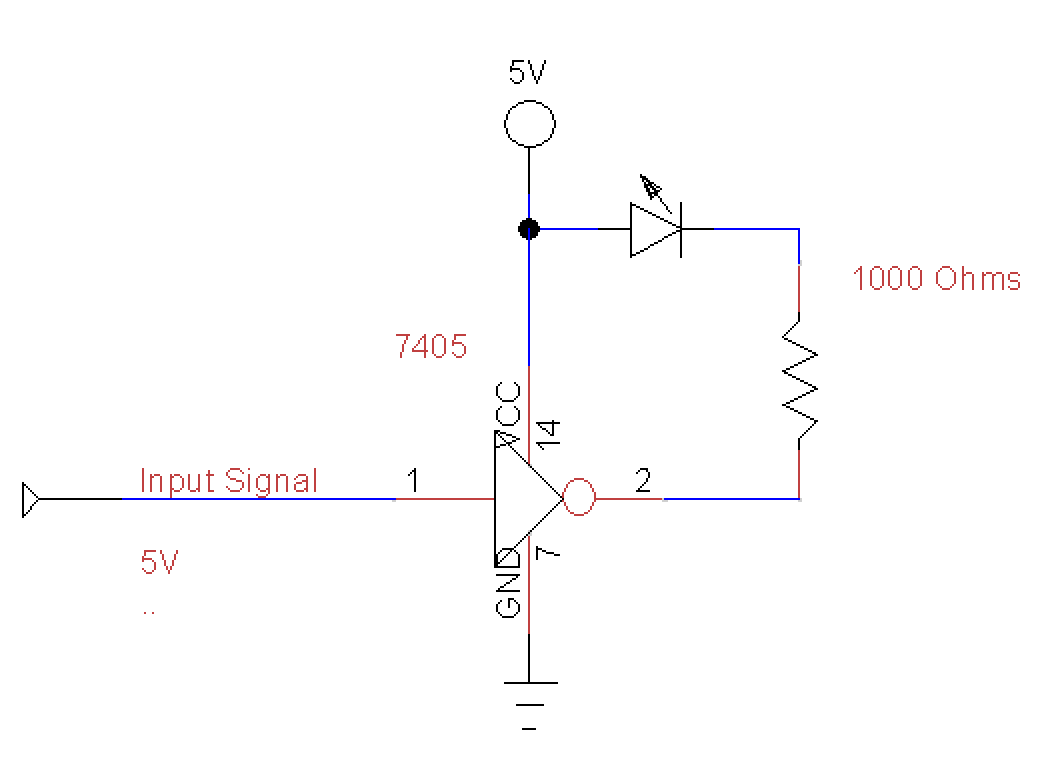
\includegraphics[scale=0.6, draft=false]{inverter}
	\caption{Controlling an LED with a LS7405 inverter.}
	\label{fig:inverter}
\end{figure}

{\em Why use a 7405, not a 7404? (ordinary inverter v. open collector inverter)}

\section{Push button debouncing}
{\em Display the debounced and non-debounced waveforms}
\begin{figure}[h]
	\centering
	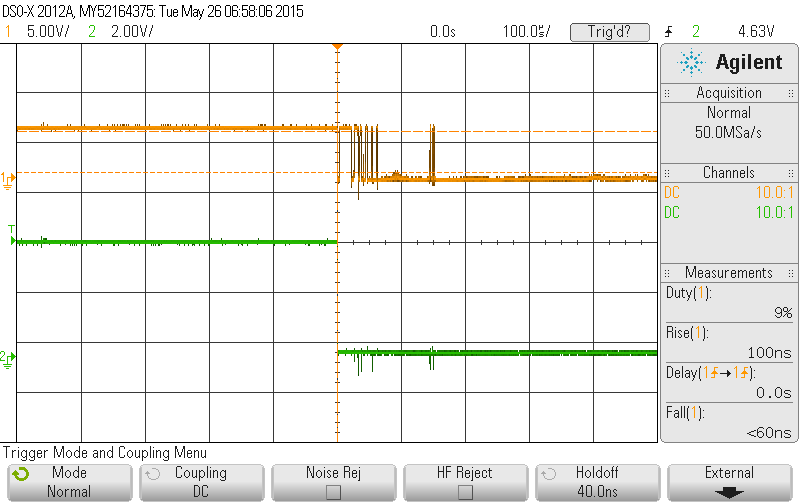
\includegraphics[width=0.95\textwidth, draft=false]{debounce}
	\caption{Waveforms of non-debounced (top) and debounced (bottom) SPDT presses}
	\label{fig:debounce}
\end{figure}

{\em Draw a debouncer with NOR gates}
\begin{figure}[h]
	\centering
	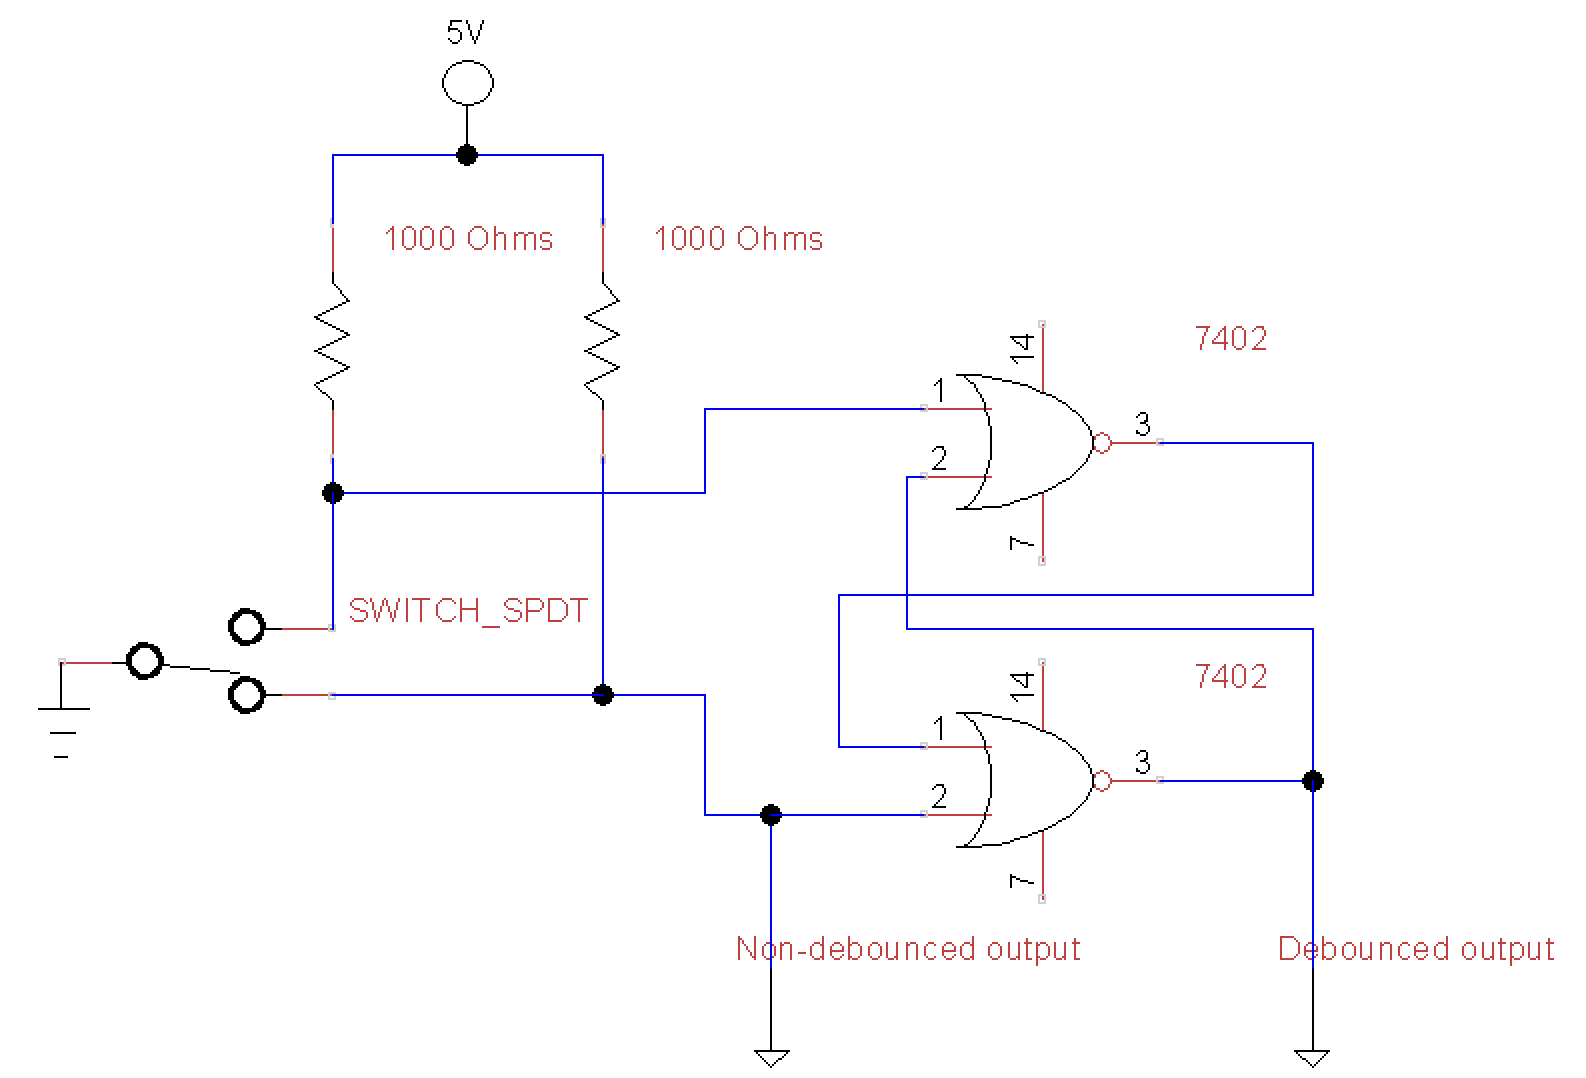
\includegraphics[scale=0.5, draft=false]{nor_gates}
	\caption{An SPDT debouncer constructed from NOR gates. For clarity, VCC and ground for gates are not connected in figure.}
	\label{fig:nor_gates}
\end{figure}

\section{Conclusion}

\end{document}